\subsection{Power Series Operations}
We now consider given a formal power series what are some things we might do with it. Recall that a power series itself is just a formal expression
$$ f(w) = a_0 + a_1w + a_2 w^2 + \dots = \sum_{n = 0}^\infty a_n w^n  $$
where $w$, rather than being a real or complex variable, is simply a formal symbol or an indeterminate. The fact that we're dealing with \textit{complex} power series simply means we allow the coefficients to be complex. Then we might ask given two power series $f(w) = \sum_{n = 0}^\infty a_n w^n$ and $g(z) = \sum_{p = 0}^\infty b_p z^p$, does $f(g(z))$ make sense? We see that
$$ f(g(z)) = a_0 + a_1(b_0 + b_1 z + \dots) + a_2(b_0 + b_1 z + \dots)^2 + \dots $$
In other words the coefficient of any $z^n$ is an infinite series. So we need to think about convergence and such to make some sense of them. But because we want to deal with power series as formal objects we also don't want to deal with all the nuances that often accompany convergence and such. However one simple restriction we can make to bypass all this is to assert $b_0 = 0$. This means the coefficient of any $z^n$ is now a finite sum which is certainly well-defined. Therefore we assert that we can compose power series $f$ with $g$ if $g$ has no constant term.

We can also define a formal derivative for power series. We write
$$f'(w) := \sum_{n = 1}^\infty n a_n w^{n - 1} = \sum_{n = 0}^\infty (n + 1) a_{n + 1} w^n$$
and define
$$ f(0) := a_0 $$

\begin{theorem}[Inverse Function Theorem for Formal Power Series]
Given a formal power series
$$f(w) = \sum_{n = 0}^\infty a_n w^n$$
there is a power series 
$$g(z) = \sum_{p = 0}^\infty b_p z^p$$
such that $b_0 = 0$ and $f \circ g = \id$ (the identity being the series $\id(z) = z$) if and only if $a_0 = 0$ and $f'(0) \neq 0$. In this case $g$ is unique and $g \circ f$ is also the identity. 

If $f$ has a positive radius of convergence, then so does $g$.
\end{theorem}
\begin{remark}
Note the similarity of the condition $f'(0) \neq 0$ to the usual inverse function theorem.
\end{remark}
\begin{proof}
We use the method of undetermined coefficients. We are are solving for $b_p$ so that
$$ a_0 + a_1(b_1z + b_2 z^2 + \dots) + a_2(b_1z + b_2 z^2 + \dots)^2 + \dots = z $$
Now we can solve for the $b_p$ by equating coefficients of $z^n$. For example, we see must have $a_0 = 0$. Moreover we see that $a_1 b_1 = 1$ which can only have a solution if $a_1 = f'(0) \neq 0 $. This shows that the condition $a_0 = 0$ and $a_1 \neq 0$ are necessary to have a solution. Conversely we see that these are sufficient to solve uniquely for the coefficents of $g$. For example, by comparing of coefficient of $z^2$ we see
$$ a_1b_2 + a_2b_1^2 = 0 $$
But since $b_1 = a_1^{-1}$ we must have $b_2 = -a_1^{-1}(a_2 b_1^2)$. Similarly we can recursively solve for all the $b_n$. This shows uniqueness of $g$.

Now note $g(0) = 0$ and $g'(0) \neq 0$ we can apply the first part of the theorem again to find $f_1(w)$ such that $g \circ f = \id$. Then
$$ f_1 = \id \circ f_1 = (f \circ g) \circ f_1 = f \circ (g \circ f_1) = f \circ \id = f $$
Note we used associativity of composition of power series. Something we have not proven but can be verified.

The argument about radius of convergence can be seen by computing estimates directly or from our usual Inverse Function Theorem (see \autoref{thm:inv-func-thm}), once we know that a holomorphic functions have Taylor series that converge and represent the function.
\end{proof}

Now that we have some understanding about formal power series let us take a look at what happens with convergence.
\begin{proposition}
If $f(w) = \sum_{n = 0}^\infty a_n w^n, g(z) = \sum_{p = 1}^\infty b_p z^p$ are convergent then so is $f \circ g$. In fact take $r > 0$ such that $\sum_{p = 1}^\infty \abs{b_p} r^p < R(f)$ where $R(f)$ is the radius of convergence for $f$. Then
\begin{enumerate}
    \item $R(f \circ g) \geq r$
    \item $\abs{g(z)} < R(f)$ if $\abs{z} < r$
    \item $f(g(z)) = (f \circ g)(z)$
\end{enumerate}
\end{proposition}
\begin{remark}
For the last point above, $f(g(z))$ involves computing $f(w)$ where $w$ is the value that $g(z)$ converges to. On other hand to compute $(f \circ g)(z)$, we first find $f \circ g$ as above and then find what value this converges to at $z$
\end{remark}
\begin{remark}
We know that an $r$ as described exists by using a simple continuity argument with $g(0) = 0$.
\end{remark}
\begin{proof}
We see that
$$ (f \circ g)(z) = \sum_{n = 0}^\infty a_n \left( \sum_{p = 0}^\infty b_p z^p \right)^n = \sum_{k = 0}^\infty c_k z^k $$
We also note that
\begin{align*}
    \abs{\sum_{n = 0}^\infty a_n \left( \sum_{p = 0}^\infty b_p z^p \right)^n} &\leq \sum_{n = 0}^\infty \abs{a_n} \left( \sum_{p = 0}^\infty \abs{b_p} \abs{z}^p \right)^n = \sum_{k = 0}^\infty \gamma_k \abs{z}^k
\end{align*}
Note that $\abs{c_k} \leq \gamma_k$. In order to see this note that $c_k$ is a polynomial in $a_0, \dots, a_k, b_1, \dots, b_k$ allowing us to write $c_k = P(a_0, \dots, a_k, b_1, \dots, b_k)$. Then $\gamma_k = P(\abs{a_0}, \dots, \abs{a_k}, \abs{b_1}, \dots, \abs{b_k})$. By the triangle inequality we conclude $\abs{c_k} \leq \gamma_k$. Then by using the limit comparison test (see \href{https://en.wikipedia.org/wiki/Limit_comparison_test#One-sided_version}{Limit comparison test}) we conclude that $(f \circ g)(z)$ converges absolutely if $\abs{z} < r$. Therefore the radius of convergence for $(f \circ g)$ is at least $r$ and moreover for such $z$ we have $\abs{g(z)} < R(f)$. The final statement is exactly an application of the fact that reordering the terms of an absolutely convergent series does not affect the sum.
\end{proof}

\begin{theorem}[Reciprocal of a power series]
If $f(z) = \sum_{n = 0}^\infty a_n z^n$ and $a_0 \neq 0$ then there is a unique power series $g(z)$ such that $f(z) g(z) = 1$. If $f$ has a positive radius of convergence then so does $g$.
\end{theorem}
\begin{proof}
We can assume that $a_0 = 1$ (we simply divide by it if necessary). Then we can write $f(z) = 1 - h(z)$ where $h(z)$ is a power series satisfying $h(0) = 0$. Then we know that $(1 - w)^{-1} = 1 + \sum_{n = 1}^\infty w^n$ so by substituting $w = h(z)$ we compute $g(z) := (1 - h(z))^{-1}$. The statement about the radius of convergence follows from the previous theorem.
\end{proof}

\section{Principal Branches}
We know that $\arg(z)$ is not well-defined on $\C$. However, we can fix this by restricting it to a subset of $\C$. The largest subset we can work with is $\C \setminus (-\infty, 0]$ on which $\arg$ has a unique value in $(-\pi, \pi)$. We call this $\text{Arg}$, the principal branch of $\arg$. 

In order to verify that $\text{Arg}$ is continuous, it suffices to show that it is continuous on $S^1 \setminus \{-1\}$. We have a continuous map $z = e^{i\theta}$ that bijectively maps $(-\pi, \pi)$ to $S^1\setminus \{-1\}$. In order to see that the inverse is continuous we can argue that the exponential map above is continuous on $[-\pi + \epsilon, \pi - \epsilon]$ for every $\epsilon > 0$. Since the domain is compact for all of these we know that the inverse maps are all going to be continuous as well. By taking smaller and smaller $\epsilon$ we eventually cover the whole space.

Since we have a principal branch for $\arg$ we can similarly have a principal branch for $\log$ which we define as $\log(\abs{z}) + i \text{Arg}(z))$. This coincides with the real log on $(0, \infty)$. 

\begin{proposition}
For $\abs{z} < 1$ the power series
$$ f(z) := \sum_{n = 1}^\infty (-1)^{n + 1} \frac{z^n}{n} $$
converges and is equal to the principal branch of $\log(1 + z)$.
\end{proposition}
\begin{proof}
One can check that $f(z)$ and $g(w) = \sum_{n = 1}^\infty \frac{w^n}{n!}$, the series expansion of $e^w - 1$, are inverses of another. Therefore $g(f(z)) = z$. This means that $e^{f(z)} = z + 1$. By definition, this means $f(z)$ is a branch of $\log(z + 1)$. We can check this is the principal branch by evaluation at $f$ at 0. 
\end{proof}

We can now define exponentiation using any complex number, not just rationals. Namely we say
$$ z^\alpha = e^{\alpha \log z} $$
for any $\alpha \in \C$ and $z \neq 0$. Note that in general this is a many-valued function of $z$ (interestingly it remains single-valued if $\alpha \in \Z$ this is because $\log z$ is only ill-defined up to integer multiplies of $2\pi$. If $\alpha$ is an integer then the power of the exponent can only vary by integer multiples of $2\pi$ but this is simply 1). 

The fact that these functions, such as $z^{1/2}$, are multi-valued can be quite difficult to handle. So instead what we would like is to have a covering space $X$ for $\C$ such that the multi-valued function lifts to a single-valued function.

For the function $w = z^{1/2}$ which we can equivalent write as $z = w^2$ there is a natural candidate for such a space. Consider $X := \{(z, w) \in \C^2 | w^2 = z\}$. This is necessary a manifold since it is the graph of a smooth function. Moreover, note the map $(z, w) \mapsto w$ on $X$ gives exactly $z^{1/2}$.

Now we want to try and think about what $X$ actually looks like. We know $X$ looks roughly like 2 copies of $\C$ since every non-zero point $z$ in $\C$ has two point $w$ so that $w^2 = z$. In particular this means that $X$ has two disjoint, homeomorphic copies of some neighbourhood of $z$ for every $z$. 

\section{Conformal mappings}
We know we can map the upper half-plane $\mathbb{H}^+$ to the open unit disk via the (conformal) map
$$ w = \frac{z - i}{z + i} $$
We now ask whether we can use conformal maps to map various different geometrical objects to one another. 

Suppose we have a circular wedge as below.\\
\begin{center}
    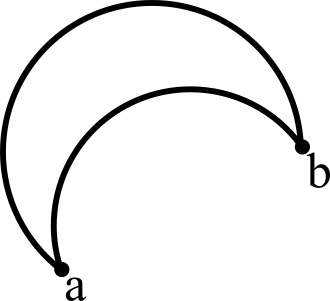
\includegraphics[scale=0.8]{Images/circular_wedge.png}
\end{center}
We ask whether or not we can map the interior of this shape to the upper half-plane and if so, how. First we can map $a$ to 0 and $b$ to infinity so that the two arcs become straight lines. We do this using
$$ \zeta = \frac{z - a}{z - b} $$
This results in an infinite wedge like shown below
\begin{center}
    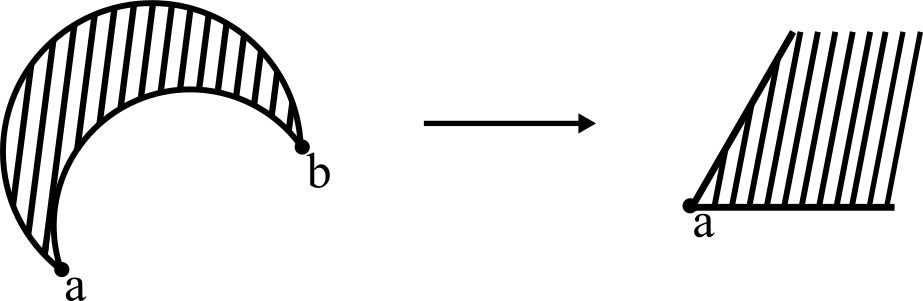
\includegraphics[scale=0.8]{Images/conformal_map.png}
\end{center}
We can then `fan' out the wedge by raising the result to some appropriate power (in particular if the angle is $\alpha$ then we rotate things so that one line lies along the positive real axis and then raise the result to the power of $\frac{\pi}{\alpha}$).

We might also have a degenerate wedge like the one below.
\begin{center}
    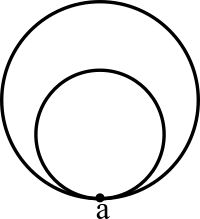
\includegraphics[scale=0.8]{Images/degenerate_wedge.png}
\end{center}
In this case we send $a$ to infinity which results in 2 parallel lines. Then we recall that $\exp$ maps $\{x + iy \in \C: x \in \R, y \in [0, \pi]\}$ to the upper half-plane which gives us the desired result.

A similar exercise is to map the complement of a line-segment to the interior (or exterior) of the unit disk, conformally. A slightly easier task to consider is how we might map this to a half-plane (we know we can go back and forth between a half-plane and a disk easily). Moreover we don't even need to have a half-plane. Given a `wedge' formed by any angle at all (like the one above) we can open or close the wedge (by raising it to some appropriate power) so that the result is a half-plane. With this in mind, we can find our conformal map quite easily.

Without loss of generality we can assume that the line segment is $[-1, 1]$ on the real line. First we do a change of coordinates
$$ z_1 = \frac{z + 1}{z - 1} $$
so that we are instead working on $\C \setminus (-\infty, 0]$. The square root function allows us to fold this into a half-plane, in this case the right half-plane (where the real part of complex numbers is positive. Then we can use
$$ w = \frac{z - 1}{z + 1} $$
to map this half-plane onto the unit disk. Overall the conformal map is $w = z - \sqrt{z^2 - 1}$.